\documentclass{standalone}

\usepackage{graphics}
\usepackage[dvipsnames,svgnames]{xcolor}

\usepackage{tikz,pgf,pgfplots,circuitikz}
\pgfplotsset{compat=1.15}
\usetikzlibrary{shapes.symbols, intersections,arrows.meta,angles,calc,3d,decorations.pathmorphing}
\usepackage[compat=1.1.0]{tikz-feynhand}

\usepackage{amssymb,amsfonts,amsthm,mathtools}
\usepackage{physics,braket,bm}

\begin{document}  

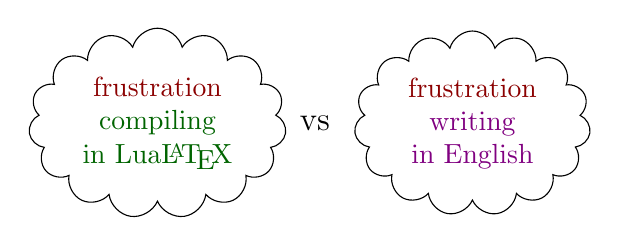
\begin{tikzpicture}
  % Define styles for the nodes
  \tikzstyle{bubble} = [draw, cloud, cloud puffs=15, cloud ignores aspect, align=center, minimum height=2cm, minimum width=3cm]
  
  % Draw the first bubble
  \node[bubble] (latex) at (1,0) {\textcolor{DarkRed}{frustration} \\ \textcolor{DarkGreen}{compiling} \\  \textcolor{DarkGreen}{in Lua{\LaTeX}}};
  
  % Draw the second bubble
  \node[bubble] (english) at (5,0) {\textcolor{DarkRed}{frustration} \\ \textcolor{Purple}{writing} \\ \textcolor{Purple}{in English}};
  
  % Draw the "vs" text in between the bubbles
  \node at (3,0) {\large vs};
\end{tikzpicture}

\end{document}
